\begin{pastexam}[label={px:ntu-115-bmei-alg-02}]{臺大生醫電資所 115 學年度 第 2 題}
（問答）

(6\%) Please draw the binary tree for the expression ``(B*(D+E)/(C-F))+ E*(A+F)'' and write prefix
and postfix forms.
\end{pastexam}

\begin{pastsoln}
答案：
\begin{itemize}
\item prefix：\texttt{+ / * B + D E - C F * E + A F}
\item postfix：\texttt{B D E + * C F - / E A F + * +}
\end{itemize}

\textbf{建樹}（資結書第~7.7~節）。 先找整個式子最後才算的運算子，它就是根，左右兩邊分別遞迴建子樹。
括號外只有 $+$ 和 $*$，$*$ 先算，所以根是中間那個 $+$：左運算元是 \texttt{(B*(D+E)/(C-F))}，右運算元
是 \texttt{E*(A+F)}。
\begin{itemize}
\item 左邊括號內是 \texttt{B*(D+E)/(C-F)}。 $*$ 和 $/$ 優先順序相同、由左往右結合，等於
\texttt{(B*(D+E))/(C-F)}，所以這棵子樹的根是 $/$，左子樹是 \texttt{B*(D+E)}（根 $*$），右子樹是 \texttt{C-F}。
\item 右邊 \texttt{E*(A+F)} 的根是 $*$，左子節點 $E$，右子樹是 \texttt{A+F}。
\end{itemize}
\begin{center}
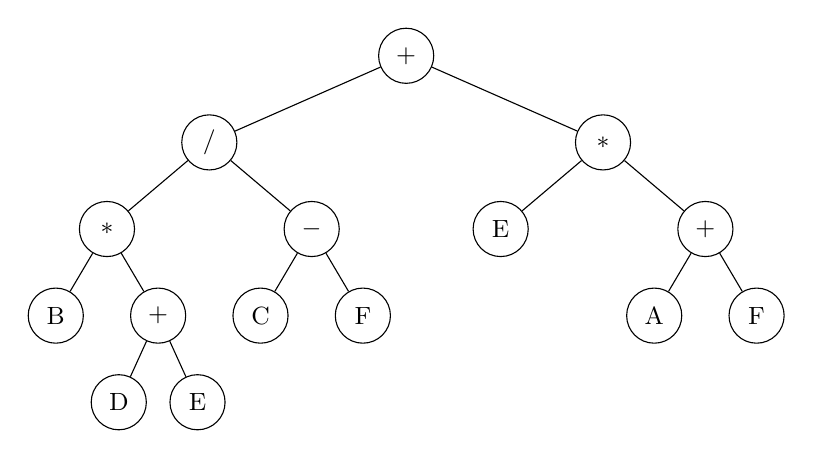
\begin{tikzpicture}[level distance=11mm,
  every node/.style={circle,draw,minimum size=7mm,inner sep=0pt,font=\small},
  level 1/.style={sibling distance=50mm}, level 2/.style={sibling distance=26mm},
  level 3/.style={sibling distance=13mm}, level 4/.style={sibling distance=10mm}]
\node {$+$}
  child {node {$/$}
    child {node {$*$}
      child {node {B}}
      child {node {$+$} child {node {D}} child {node {E}}}}
    child {node {$-$}
      child {node {C}}
      child {node {F}}}}
  child {node {$*$}
    child {node {E}}
    child {node {$+$}
      child {node {A}}
      child {node {F}}}};
\end{tikzpicture}
\end{center}
葉節點都是運算元，內部節點都是運算子，括號不出現在樹裡：結合的順序已經由樹的形狀表示了。

\textbf{前序}（根、左、右）和\textbf{後序}（左、右、根）照資結書虛擬碼~7.1 走訪：
\begin{itemize}
\item 前序：先寫根 $+$，再走左子樹 \texttt{/ * B + D E - C F}，再走右子樹 \texttt{* E + A F}，
合起來是 \texttt{+ / * B + D E - C F * E + A F}。
\item 後序：左子樹 \texttt{B D E + * C F - /}，右子樹 \texttt{E A F + *}，最後是根 $+$，合起來是
\texttt{B D E + * C F - / E A F + * +}。
\end{itemize}
檢查後序：用堆疊由左往右求值，\texttt{D E +} 得 $D+E$，\texttt{B} 和它做 $*$ 得 $B(D+E)$，\texttt{C F -}
得 $C-F$，再做 $/$ 得 $B(D+E)/(C-F)$；\texttt{E A F + *} 得 $E(A+F)$；最後 $+$，就是原式。 前序也可以從
右往左用堆疊同樣檢查（資結書第~6.3.5~節）。
\end{pastsoln}
